\documentclass[12pt]{article}
\usepackage[margin = 1in]{geometry}
\usepackage{amsmath}
\usepackage{graphicx}
\graphicspath{{./}}

\newcommand{\acos}{\text{cos}^{-1}}
\newcommand{\asin}{\text{sin}^{-1}}
\newcommand{\atan}{\text{tan}^{-1}}
\newcommand{\acosh}{\text{cosh}^{-1}}
\newcommand{\asinh}{\text{sinh}^{-1}}
\newcommand{\atanh}{\text{tanh}^{-1}}
\newcommand{\oder}{\hspace{5mm}\text{or}\hspace{5mm}}

\begin{document}
\begin{table}[h]
\centering
\begin{tabular}{c | l | c}
Symbol & Meaning & Value \\ \hline \hline
$\zeta(3)$ & Apery's constant & 1.202...\\ \hline
$B$ & Backhouse's constant & 1.456...\\ \hline
$e$ & Base of the natural logarithm & 2.718...\\ \hline
$K$ & Catalan's constant & 0.915...\\ \hline
$\pi$ & Circle constant & 3.141...\\ \hline
$\gamma$ & Euler-Mascheroni constant & 0.577...\\ \hline
$\alpha$ & Feigenbaum's alpha & 2.502...\\ \hline
$\delta$ & Feigenbaum's delta & 4.669...\\ \hline
$\xi$ & Foias constant & 1.187... \\ \hline
$F$ & Frans\'en-Robinson constant & 2.807...\\ \hline
$G$ & Gauss's constant & 0.834...\\ \hline
$A$ & Glaisher-Kinkelin constant & 1.282...\\ \hline
$\phi$ & Golden ratio & 1.618... \\ \hline
$\eta$ & Grossman's constant & 0.737... \\ \hline
$\rho$ & Kepler-Bouwkamp constant & 0.114...\\ \hline
$K_{0}$ & Khinchin's constant & 2.685...\\ \hline
$q$ & Komornik-Loreti constant & 1.787...\\ \hline
$K_{LR}$ & Landau-Ramanujan constant & 0.764...\\ \hline
$L$ & Lemniscate constant & 2.622...\\ \hline
$M_{3}$ & Madelung constant & -1.747...\\ \hline
$M$ & Meissel-Mertens constant & 0.261...\\ \hline
$C$ & Niven's constant & 1.705...\\ \hline
$\Omega$ & Omega constant & 0.567...\\ \hline
$\sigma_{p}$ & Paper folding constant & 0.850... \\ \hline
$\mu$ & Ramanujan-Soldner constant & 1.451...\\ \hline
$\psi$ & Reciprocal Fibonacci constant & 3.359...\\ \hline
$\sigma$ & Somos' quadratic recurrence constant & 1.661...\\ \hline
$\Pi_{2}$ & Twin primes constant & 0.660...\\ \hline
$P$ & Universal parabolic constant & 2.295...\\ \hline
\end{tabular}
\end{table}

\section*{Constant Definitions}

\subsection{Backhouse's Constant, $B$}
Let $p_{k}$ be the $k$th prime. Let
\begin{equation*}
P(x) = 1 + \sum_{k = 1}^{\infty} p_{k}x^{k}
\end{equation*}
and in turn let
\begin{align*}
Q(x) &= \frac{1}{P(x)}\\
&= \sum_{k = 0}^{\infty} q_{k}x^{k}.
\end{align*}
Then Backhouse's constant is given by
\begin{equation*}
B = \lim_{k \rightarrow \infty} \left| \frac{q_{k + 1}}{q_{k}} \right|.
\end{equation*}

\subsection{The Base of the Natural Logarithm, $e$}
The base of the natural logarithm.

\subsection{Catalan's Constant, $K$}
\begin{equation*}
K = \sum_{n = 0}^{\infty} \frac{(-1)^{n}}{(2n + 1)^{2}}
\end{equation*}

\subsection{The Circle Constant, $\pi$}
The ratio of a circle's circumference to its diameter.

\subsection{The Euler-Mascheroni Constant, $\gamma$}
\begin{equation*}
\gamma = \lim_{n \rightarrow \infty} \left( -\ln(n) + \sum_{k = 1}^{n} \frac{1}{k} \right)
\end{equation*}

\subsection{Feigenbaum's $\alpha$ and $\delta$ Constants}
Consider a species where the population of one generation depends on the population of the prior generation according to the recurrence relation
\begin{equation*}
P_n = r P_{n-1} \left( 1 - P_{n-1} \right)
\end{equation*}
where $r$ is a constant parameter. As $n$ goes to $\infty$, you might expect the population to settle on an equilibrium value. The value of the parameter $r$ controls what this equilibrium value is. For many values of $r$, we see the population settle on a single value. However, for other values, the population may cycle back and forth between two or three (or more) values with successive generations. This behavior can be visualized in a bifurcation plot, like Figure \ref{figure:bif}.

When $r$ is less than one, the population drops every generation, settling on 0, as seen in the plot. When $r$ is about 2, the population settles near 0.5. When $r$ is 3.2, the population will vacillate between two different sizes with successive generations. At 3.5, we cycle between four different sizes. If we pay attention to the values of $r$ at which these splits (bifurcations) happen, we can find the $\delta$ constant. 

If three consecutive bifurcations occur at $r$ values of $r_n$, $r_{n+1}$, and $r_{n+2}$, then let the lengths 
\begin{align*}
L_n &= r_{n+1} - r_n \text{ and}\\
L_{n+1} &= r_{n+2} - r_{n+1}.
\end{align*}
We then get
\begin{equation*}
\delta = \lim_{n \rightarrow \infty}\frac{L_n}{L_{n+1}}.
\end{equation*}
The $\alpha$ constant is found similarly. When a bifurcation occurs, two ``tines" arise. If we then increase $r$ until just before the next bifurcation occurs, we can record the distance between the tips of those two tines. The ratio of these distances for successive bifurcations converges to the $\alpha$ constant.
\begin{figure}[h]
\centering
\caption{Bifurcation diagram for the logistic map}
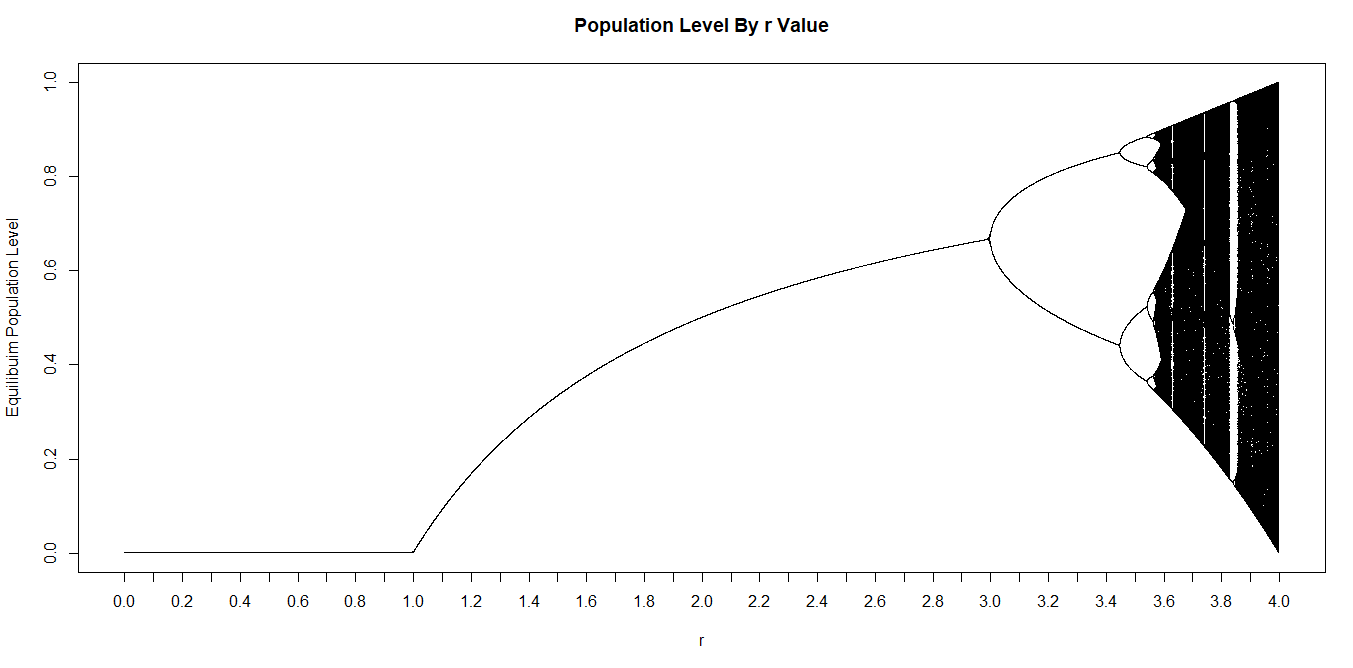
\includegraphics[scale=0.5]{pop_by_r.png}
\label{figure:bif}
\end{figure}

\subsection{Foias Constant, $\xi$}
Let $x_{1} > 0$ and
\begin{equation*}
x_{n+1} = \left(1 + \frac{1}{x_{n}}\right)^{n}.
\end{equation*}
Then there is exactly one value of $x_{1} = \xi$ such that $x_{n} \rightarrow \infty$.

\subsection{The Frans\'en-Robinson Constant, $F$}
\begin{equation*}
F = \int_{0}^{\infty} \frac{dx}{\Gamma(x)}
\end{equation*}
Where
\begin{equation*}
\Gamma(x) = \int_{0}^{\infty} t^{x - 1}e^{-t} dt 
\end{equation*}

\subsection{Gauss's Constant, $G$}
\begin{equation*}
G = \frac{1}{\operatorname{agm}(1,\sqrt{2})}
\end{equation*}
Where $\operatorname{agm}(a,b)$ is the arithmetic-geometric mean of $a$ and $b$.

\subsection{The Golden Ratio, $\phi$}
The greater of the two solutions to $x^{2} = x + 1$, namely
\begin{equation*}
\frac{1 + \sqrt{5}}{2}.
\end{equation*}

\subsection{Grossman's Constant, $\eta$}
Define the sequence $a_{0} = 1$, $a_{1} = x$, and
\begin{equation*}
a_{n} = \frac{a_{n-2}}{1 + a_{n-1}}.
\end{equation*}
This sequence converges for exactly one value of $x = \eta$.

\subsection{The Kepler-Bouwkamp Constant, $\rho$}
\begin{equation*}
\rho = \prod_{k = 3}^{\infty} \cos\left( \frac{\pi}{k} \right)
\end{equation*}

\subsection{Khinchin's Constant, $K_{0}$}
The coefficients of the continued fraction expansion of a real number almost always have a finite geometric mean which converges to this constant. That is, if 
\begin{equation*}
x = a_{0} + \frac{1}{a_{1} + \frac{1}{a_{2} + \cdots}},
\end{equation*}
then it is almost always true that
\begin{equation*}
\lim_{n \rightarrow \infty}(a_{1} a_{2} \ldots a_{n})^{1/n} = K_{0}.
\end{equation*}

\subsection{The Komornik-Loreti Constant, $q$}
The Thue-Morse sequence is defined by the recurrence relation
\begin{align*}
t_{0} &= 0\\
t_{2n} &= t_{n}\\
t_{2n+1} &= 1 - t_{n}
\end{align*}
The Komornik-Loreti constant, $q$, is the solution to
\begin{equation*}
1 = \sum_{n=1}^{\infty} \frac{t_{n}}{q^{n}}
\end{equation*}

\subsection{The Meissel-Mertens Constant, $M$}
The value of the limit
\begin{equation*}
\lim_{n \rightarrow \infty} \left( -\ln\left( \ln(n) \right) + \sum_{p \leq n} \frac{1}{p} \right)
\end{equation*}
for primes $p$. 

\subsection{Niven's Constant, $C$}
If the prime factorization of an integer $m$ is written as
\begin{equation*}
m = (p_{1}^{a_{1}})(p_{2}^{a_{2}})(p_{3}^{a_{3}}) \ldots ,
\end{equation*}
then we define the function $H$ as
\begin{equation*}
H(m) = \max(a_{1},\: a_{2},\: a_{3}, \ldots) .
\end{equation*}
Niven's constant is then given by the limit
\begin{equation*}
C = \lim_{n \rightarrow \infty} \frac{1}{n} \sum_{m = 1}^{n} H(m) .
\end{equation*}
So $C$ is the ``average" greatest number of times a prime occurs in the prime factorization of an integer.

\subsection{The $\Omega$ Constant}
The solution to
\begin{equation*}
x e^{x} = 1 .
\end{equation*}

\subsection{The Paper Folding Constant, $\sigma_{p}$}
Take a strip of paper and fold it in half, right over left, infinitely often. Upon unfolding it, assign each ``valley" crease a 1, and each ``mountain" crease a 0. That sequence begins:
\begin{equation*}
a = \{1,1,0,1,1,0,0,1,1,1,0,0,1,0,0, \ldots\}
\end{equation*}
Then,
\begin{equation*}
\sigma_{p} = \sum_{n=1}^{\infty} \frac{a_{n}}{2^{n}}
\end{equation*}

\subsection{The Ramanujan-Soldner Constant, $\mu$}
The Ramanujan-Soldner constant, $\mu$, is the unique positive solution to
\begin{equation*}
\int_{0}^{x} \frac{dt}{\ln(t)} = 0
\end{equation*}

\subsection{The Reciprocal Fibonacci Constant, $\psi$}
The value of the summation
\begin{equation*}
\sum_{n = 1}^{\infty} \frac{1}{F_{n}}
\end{equation*}
where $F_{n}$ is the $n$th Fibonacci number.

\subsection{Somos' Quadratic Recurrence Constant, $\sigma$}
\begin{align*}
\sigma &= \sqrt{1 \sqrt{2 \sqrt{3\cdots} }}\\
&= \prod_{n = 1}^{\infty} \left( \frac{1 + n}{n} \right)^{2^{-n}}
\end{align*}

\subsection{The Universal Parabolic Constant, $P$}
The latus rectum of a parabola is the line segment whose end points lie on the parabola and which passes through its focus parallel to its directrix. The focal parameter of a parabola is the distance from its directrix to its focus. Let $A$ be the arc length of the parabolic segment formed by the latus rectum of a parabola and $p$ be the focal parameter of that parabola. The the universal parabolic constant is
\begin{align*}
P &= \frac{A}{p}\\
&= \ln(1 + \sqrt{2}) + \sqrt{2}.
\end{align*}

\pagebreak
\section{January}
\begin{align*}
1.01 &= \sqrt[K]{e-C}\\
1.02 &= -\left(\frac{M_{3}}{C}\right)\\
1.03 &= \csc{(\gamma \pi)}\\
1.04 &= \mu^{\rho}\\
1.05 &= \sqrt[\sigma]{\frac{1}{K}}\\
1.06 &= \cosh\left(\sqrt[M]{K_{LR}}\right)\\
1.07 &= \frac{1}{\gamma \phi}\\
1.08 &= \ln\left(\cosh\left(M_{3}\right)\right)\\
1.09 &= \frac{1}{K}\\
1.10 &= \gamma^{\ln\left(G\right)} \oder \tan(G)\\
1.11 &= P\log_{G}\left(K\right)\\
1.12 &= \sqrt{P - \ln(F)} \oder \gamma - \ln(\gamma) \oder \cosh^{-1}(C)\\
1.13 &= \ln^{\gamma}\left(\pi + \frac{1}{\pi}\right)\\
1.14 &= \ln\left(\phi \cosh(A)\right) \oder \sinh\left(\tanh(P)\right)\\
1.15 &= \left(1 + \sqrt[\left(e-\pi\right)]{e}\right)^{\phi}\\
1.16 &= \frac{e \sqrt[\phi]{\phi}}{\pi}\\
1.17 &= \sec(\ln \gamma)\\
1.18 &= \phi - \frac{1}{2\ln\pi}\\
1.19 &= \atan{\alpha} \oder \frac{\sqrt{2}}{\xi} \oder \sqrt[e]{\phi}\\
1.20 &= \zeta(3) \oder \frac{\ln{2}}{\gamma} \oder \sqrt{\mu}\\
1.21 &= \ln{\psi} \oder \atan{K_{0}}\\
1.22 &= \frac{\mu}{\xi} \oder \frac{\sqrt{\pi\,}}{\mu}\\
1.23 &= \sqrt{\frac{1}{\Pi_{2}}} \oder \sqrt{\pi-\phi\,}\\
1.24 &= \frac{1}{\sinh{\eta}}\\
\end{align*}
\begin{align*}
1.25 &= \sqrt{1+\Omega\,} \oder \frac{\pi}{\alpha}\\
1.26 &= e-B \oder \csc\left(K\right)\\
1.27 &= \gamma + \ln{2} \oder K_{0}-\sqrt{2} \oder \sqrt{\phi}\\
1.28 &= A \oder \log_{B}(\phi)\\
1.29 &= \cosh\left(\sigma-K\right) \oder \atan\left(e A\right)\\
1.30 &= \frac{\acosh \phi}{\gamma \sqrt{2}} \oder \tan{K}\\
1.31 &= \ln\left(\phi P\right) \oder \frac{\zeta(3)}{K}\\
\end{align*}

\pagebreak

\section{February}
\begin{align*}
2.01 &= \sqrt[\xi]{P} \oder \acosh\left(1+F\right)\\
2.02 &= A \left(\gamma+1\right) \oder \Omega+B\\
2.03 &= \sqrt{\phi+\alpha}\\
2.04 &= \sqrt{B+e} \oder \frac{L}{A}\\
2.05 &= \mu \sqrt{2} \oder \log_{\phi}\left(K_{0}\right)\\
2.06 &= \frac{L}{\sqrt{\phi\,}}\\
2.07 &= e^{\gamma^{\gamma}} \oder \pi \Pi_{2}\\
2.08 &= \acosh\left(\mu F\right) \oder \sqrt{\xi+\pi} \\
2.09 &= \frac{\mu}{\ln{2}}\\
2.10 &= e-\frac{1}{\phi} \oder \frac{B}{\ln{2}}\\
2.11 &= \frac{\gamma}{\sigma_{p}-\gamma} \oder \sqrt{C L}\\
2.12 &= B^{2} \oder \ln\left(\tan{\mu}\right)\\
2.13 &= \acos\left(\frac{1}{G-e}\right) \oder \sqrt[K]{2\,}\\
2.14 &= \frac{\sqrt{2}}{\Pi_{2}}\\
2.15 &= e-\Omega\\
2.16 &= \sqrt{\delta\,} \oder \delta-\alpha\\
2.17 &= \cos\left(M\right)+\atan\left(L\right)\\
2.18 &= \sqrt[A]{e} \oder \frac{1 + e}{C}\\
2.19 &= \frac{1}{B-1}\\
2.20 &= \sqrt{\pi \ln{\delta}}\\
2.21 &= \pi^{\ln(2)}\\
2.22 &= \cosh^{-1}\left(\delta\right) \oder \phi^{\sigma}\\
2.23 &= \left(1+\Omega\right)^{q} \oder \log_{\mu}\left(P\right)\\
2.24 &= \sqrt[\sigma]{\frac{1}{M}}\\
2.25 &= \sqrt{\alpha+K+\sigma}\\
2.26 &= \frac{e}{\zeta(3)}\\
\end{align*}
\begin{align*}
2.27 &= q^{\sqrt{2}}\\
2.28 &= K_{0}^{G}\\
2.29 &= P\\
\end{align*}

\pagebreak

\section{March}
\begin{align*}
3.01 &= \phi^{\alpha K}\\
3.02 &= \phi^{B + \sin(1)}\\
3.03 &= \frac{1}{\rho - \cos(q)}\\
3.04 &= \frac{\pi}{\ln F}\\
3.05 &= \delta - \phi\\
3.06 &= \phi + \frac{1}{\ln 2} \oder \pi^{\sqrt[4]{K}}\\
3.07 &= \alpha+\Omega\\
3.08 &= \delta \Pi_{2} \oder L+\frac{B}{\pi}\\
3.09 &= P^{\frac{e}{2}}\\
3.10 &= \pi \ln{K_{0}}\\
3.11 &= \log_{\mu}\left(L+\Omega\right)\\
3.12 &= -\frac{\ln \pi}{\ln(\ln 2)}\\
3.13 &= K_{0}^{\frac{\pi}{e}}\\
3.14 &= \pi \oder \zeta(3)+\frac{\phi}{G}\\
3.15 &= \gamma+\sqrt[A]{\psi}\\
3.16 &= C + B \oder \pi B-\sqrt{2}\\
3.17 &= \frac{\alpha}{C - K}\\
3.18 &= e^{\sin^{-1}(K)} \oder \sqrt{\pi} + \sqrt{2}\\
3.19 &= P \sqrt{\sinh\sqrt{2}} \oder K_{0} \sqrt[4]{2}\\
3.20 &= \sqrt[e]{\frac{e}{\rho}} \oder \frac{1}{e \rho}\\
3.21 &= \frac{\delta\sqrt{\gamma+\Pi_{2}}}{\phi} \oder K+P\\
3.22 &= \pi-\ln\left(\tanh\phi\right)\\
3.23 &= \delta-\sqrt[e]{K_{0}} \oder \frac{\tan B}{K_{0}}\\
3.24 &= q\cosh(\zeta(3)) \oder B+q\\
3.25 &= \cosh\left(\xi+\Pi_{2}\right) \oder B^{\pi}\\
3.26 &= F^{\ln\pi} \oder \eta^{2} + e\\
\end{align*}
\begin{align*}
3.27 &= \asinh\left((\gamma + F)\sqrt[\eta]{e\,}\right) \oder \xi A-M_{3}\\
3.28 &= e\sqrt{B\,} \oder \sigma+\sqrt{L}\\
3.29 &= e-\frac{1}{M_{3}} \oder e+\gamma\\
3.30 &= \frac{e}{\tan\left(\frac{1}{\mu}\right)} \oder \frac{F}{\sigma_{p}}\\
3.31 &= \sqrt{A\,}+\cosh\sqrt{2\,} \oder L+\frac{1}{\mu}\\
\end{align*}

\pagebreak

\section{April}
\begin{align*}
4.01 &= **\\
4.02 &= **\\
4.03 &= **\\
4.04 &= **\\
4.05 &= **\\
4.06 &= **\\
4.07 &= **\\
4.08 &= **\\
4.09 &= **\\
4.10 &= **\\
4.11 &= **\\
4.12 &= **\\
4.13 &= **\\
4.14 &= **\\
4.15 &= **\\
4.16 &= **\\
4.17 &= **\\
4.18 &= **\\
4.19 &= **\\
4.20 &= **\\
4.21 &= **\\
4.22 &= **\\
4.23 &= **\\
4.24 &= **\\
4.25 &= **\\
4.26 &= **\\
4.27 &= **\\
4.28 &= **\\
4.29 &= **\\
4.30 &= **\\
\end{align*}

\pagebreak

\section{May}
\begin{align*}
5.01 &= **\\
5.02 &= **\\
5.03 &= **\\
5.04 &= **\\
5.05 &= **\\
5.06 &= **\\
5.07 &= **\\
5.08 &= **\\
5.09 &= **\\
5.10 &= **\\
5.11 &= **\\
5.12 &= \sigma^{\delta / \mu} \oder \pi + \Omega + \sqrt{2}\\
5.13 &= -\tan\left(\frac{1}{\Omega}\right)\\
5.14 &= K_{0}^{\cosh^{-1}(e)} \oder e^{\sqrt{K_{0}}}\\
5.15 &= \alpha^{q} \oder \frac{\tan(\mu)}{\phi} \oder \delta\tan(G)\\
5.16 &= **\\
5.17 &= **\\
5.18 &= **\\
5.19 &= **\\
5.20 &= **\\
5.21 &= **\\
5.22 &= **\\
5.23 &= **\\
5.24 &= **\\
5.25 &= **\\
5.26 &= **\\
5.27 &= **\\
5.28 &= **\\
5.29 &= **\\
5.30 &= **\\
5.31 &= **\\
\end{align*}

\pagebreak

\section{June}
\begin{align*}
6.01 &= **\\
6.02 &= **\\
6.03 &= **\\
6.04 &= **\\
6.05 &= **\\
6.06 &= **\\
6.07 &= **\\
6.08 &= **\\
6.09 &= **\\
6.10 &= **\\
6.11 &= **\\
6.12 &= **\\
6.13 &= **\\
6.14 &= **\\
6.15 &= **\\
6.16 &= **\\
6.17 &= **\\
6.18 &= **\\
6.19 &= **\\
6.20 &= **\\
6.21 &= **\\
6.22 &= **\\
6.23 &= **\\
6.24 &= **\\
6.25 &= **\\
6.26 &= **\\
6.27 &= **\\
6.28 &= **\\
6.29 &= **\\
6.30 &= **\\
\end{align*}

\pagebreak
 
\section{July}
\begin{align*}
7.01 &= **\\
7.02 &= **\\
7.03 &= **\\
7.04 &= **\\
7.05 &= **\\
7.06 &= **\\
7.07 &= **\\
7.08 &= **\\
7.09 &= **\\
7.10 &= **\\
7.11 &= **\\
7.12 &= **\\
7.13 &= **\\
7.14 &= **\\
7.15 &= **\\
7.16 &= **\\
7.17 &= **\\
7.18 &= **\\
7.19 &= **\\
7.20 &= **\\
7.21 &= **\\
7.22 &= **\\
7.23 &= **\\
7.24 &= **\\
7.25 &= **\\
7.26 &= **\\
7.27 &= \pi^{\rho + \phi}\\
7.28 &= e^{\sqrt{K_{0}}}\sqrt{2}\\
7.29 &= \frac{G}{\tanh(\rho)}\\
7.30 &= \sqrt{\sinh(\delta)}\\
7.31 &= \alpha^{\sigma} + e \oder C e^{B}\\
\end{align*}

\pagebreak
 
\section{August}
\begin{align*}
8.01 &= **\\
8.02 &= **\\
8.03 &= \ln(2)\cosh(\pi)\\
8.04 &= e^{\sqrt{\phi K_{0}}}\\
8.05 &= \frac{\alpha K_{0}}{G}\\
8.06 &= \sinh\left(\frac{\psi}{\sqrt{B}}\right)\\
8.07 &= \sinh\sqrt{\sigma \delta}\\
8.08 &= **\\
8.09 &= **\\
8.10 &= B^{\frac{B}{M}} \\
8.11 &= \phi^{\frac{1}{2\rho}} \oder \alpha^{A + 1}\\
8.12 &= \frac{\alpha^{\psi}}{K_{0}} \oder \delta^{\frac{e}{2}}\\
8.13 &= -\frac{K_{0} M_{3}}{\gamma} \oder -\tan(1 + \ln(2))\\
8.14 &= e^{P} - q \\
8.15 &= **\\
8.16 &= **\\
8.17 &= e^{\frac{B}{\ln(2)}} \\
8.18 &= K_{0} \log_{B}(\pi) \oder \left(\sinh^{-1}P\right)^{\delta}\\
8.19 &= 2^{\frac{\sinh \alpha}{2}} \oder \sigma^{\psi} + K_{0}\\
8.20 &= \cosh(F) - \rho \oder \frac{\log_{\phi}F}{M}\\
8.21 &= \alpha^{P} \oder K+\sinh(K_{0}) \\
8.22 &= **\\
8.23 &= \left(\frac{\pi}{2}\right)^{\delta} \oder e^{(K + F)^{\Omega}}\\
8.24 &= B^{q \pi} \oder e \log_{\sigma}(\delta)\\
8.25 &= \sinh(F) \oder \log_{K}\left(\frac{1}{e}\right) - \pi\\
\end{align*}
\begin{align*}
8.26 &= \frac{K e}{\rho L} \oder \psi - F M_{3}\\
8.27 &= \delta \sqrt{\pi} \oder e^{\mu B} \oder \frac{-\log(\rho)}{M}\\
8.28 &= \frac{q - G}{\rho}\\
8.29 &= **\\
8.30 &= **\\
8.31 &= \cosh(F) \oder K - \tan(C) \oder \psi^{-M_{3}}\\
\end{align*}

\pagebreak
 
\section{September}
\begin{align*}
9.01 &= \cosh(B)^{\gamma \delta} \oder \pi^{\phi}\sqrt{2}\\
9.02 &= \pi F^{G^{(\alpha - L)}} \oder \psi K_{0}\\
9.03 &= C^{P^{C}}\\
9.04 &= \sqrt[\Omega]{e A} \oder \sigma^{\frac{\alpha}{\gamma}} \oder \psi^{\frac{e + K}{2}}\\
9.05 &= **\\
9.06 &= **\\
9.07 &= **\\
9.08 &= **\\
9.09 &= **\\
9.10 &= **\\
9.11 &= **\\
9.12 &= **\\
9.13 &= **\\
9.14 &= \delta+K_{0}+q \oder \ln(\psi) \sinh(e)\\
9.15 &= B+\sqrt[M]{C} \oder \frac{F}{1-\ln(2)} \oder e \left(\sigma+C\right)\\
9.16 &= K_{0} \left(e+\ln{2}\right) \oder \phi+\sinh(e)\\
9.17 &= \phi(1 + \delta) \oder \sigma \delta+\sqrt{2} \oder Fe\zeta(3)\\
9.18 &= \cosh(B+\mu)\\
9.19 &= \mu \sqrt[G]{\delta} \oder \mu \tan\left(\sqrt{2}\right)\\
9.20 &= \sqrt[\pi]{\rho}+\frac{1}{\rho} \oder (\mu + \pi)^{B}\\
9.21 &= \delta+\phi F \oder \sqrt[M]{q}\\
9.22 &= \psi^{\sqrt{\psi}} \oder \frac{\pi \psi}{\ln \pi}\\
9.23 &= \frac{\acosh(\phi)}{\rho} \oder \frac{1}{\rho}+\ln C\\
9.24 &= \frac{1}{\rho}+\asinh\Omega\\
9.25 &= \sinh(\pi)-P \oder \sqrt[q]{\sinh(\delta)}\\
\end{align*}
\pagebreak
\begin{align*}
9.26 &= \frac{1}{\frac{1}{\pi}+\mu-\sigma} \oder \frac{\sinh(\phi)}{M}\\
9.27 &= \gamma+\frac{1}{\rho} \oder \sinh\left(\psi-\frac{\xi}{e}\right)\\
9.28 &= e+\alpha L \oder \frac{\pi C}{\gamma}\\
9.29 &= (\delta+1) \sqrt{K_{0}} \oder \pi \cosh\left(M_{3}\right)\\
9.30 &= P(\psi + \ln2) \oder \pi e \sqrt{\xi\,} \\
\end{align*}

\pagebreak
 
\section{October}
\begin{align*}
10.01 &= \frac{1+\phi}{M}\\
10.02 &= \frac{e^2}{\eta} \oder \frac{L}{M}\\
10.03 &= \pi^{\csc(L)}\\
10.04 &= \frac{B}{\rho}-L \oder \alpha+\sinh\left(e\right)\\
10.05 &= \tan\left(\frac{G}{\Omega}\right) \oder \frac{\sec \mu}{G}\\
10.06 &= \frac{\cosh P}{-K + \sqrt{2}}\\
10.07 &= \delta+e+K_{0} \oder B \cosh L\\
10.08 &= \sinh\left(\frac{C}{\Omega}\right) \oder \cosh\left(\sqrt[G]{\alpha}\right)\\
10.09 &= \frac{\zeta\left(3\right)}{\rho}-\frac{1}{e} \oder \sinh\left(\delta-\sigma\right)\\
10.10 &= -\frac{\phi^2 \sqrt{2\,}}{\ln \ln 2} \oder e(e + 1)\\
10.11 &= \frac{1}{\rho} + \sqrt{2\,}\\
10.12 &= \frac{\mu}{\rho} - \alpha\\
10.13 &= \sqrt[\Omega]{\gamma+\pi}\\
10.14 &= \cosh\left(\delta-\sigma\right)\\
10.15 &= \frac{e}{\atanh{M}}\\
10.16 &= \sinh\left(\alpha + \sqrt{M}\right)\\
10.17 &= \frac{\xi + \sqrt{2}}{\atan M}\\
10.18 &= \tan(\acosh P)\\
10.19 &= (\sigma + \ln 2)(\pi + \xi)\\
10.20 &= \frac{\delta}{\Pi_{2} \ln 2}\\
10.21 &= \sqrt[-\gamma]{M}\\
\end{align*}
\begin{align*}
10.22 &= \frac{K_{0} F}{\eta}\\
10.23 &= L + \cosh{(e)}\\
10.24 &= L (e + \xi) \oder e + \sqrt[\Omega]{\pi}\\
10.25 &= \psi \csc(F)\\
10.26 &= e + \sinh(e) \oder e \pi \zeta(3)\\
10.27 &= \frac{1}{G - \eta} \oder \frac{e}{\asin{M}}\\
10.28 &= \frac{\phi \sigma}{M}\\
10.29 &= \zeta(3)^{B/\rho}\\
10.30 &= \frac{e}{\rho P}\\
10.31 &= P^{F}\\
\end{align*}

\pagebreak
 
\section{November}
\begin{align*}
11.01 &= q^{e + \sqrt{2}}\\
11.02 &= q (\psi + F)\\
11.03 &= \sinh(\pi)\atan\sqrt{2} \oder e+\cosh{F}\\
11.04 &= \frac{\pi^{\phi}}{\gamma} \oder \frac{F \delta}{\xi}\\
11.05 &= \left(\Pi_{2} + \delta\right) \sqrt[\sigma]{\psi\,}\\
11.06 &= L \sqrt[\gamma]{P}\\
11.07 &= (\pi+\ln 2)\log_{C}(\delta)\\
11.08 &= \cosh\left(\frac{q}{\gamma}\right)\\
11.09 &= \frac{\psi \delta}{\sqrt{2}}\\
11.10 &= \frac{\alpha}{\ln(B)\tanh(\ln 2)}\\
11.11 &= BFe\\
11.12 &= \Omega M-\tan(\sigma)\\
11.13 &= \gamma+\psi \pi\\
11.14 &= \psi \sqrt[\ln(2)]{P}\\
11.15 &= F^{\frac{F}{\zeta(3)}} \oder \frac{A}{\rho}\\
11.16 &= L + \pi e \oder L^{\alpha}\\
11.17 &= \frac{1}{F-e}\\
11.18 &= \sinh(\pi)-\frac{1}{e}\\
11.19 &= \frac{e^{2}}{\Pi_{2}}\\
11.20 &= \left(\frac{F}{\xi}\right)^{F} \oder (\delta+e)\sqrt[A]{C} \\
11.21 &= \frac{L \sinh\left(\sqrt{L}\right)}{\Omega}\\
11.22 &= \frac{\sinh e}{\sin\eta} \oder \psi + \pi\alpha\\
11.23 &= \psi P B\\
11.24 &= \tan\left(\phi K\right)\\
11.25 &= \cosh(e \ln \pi)\\
\end{align*}
\begin{align*}
11.26 &= \cosh\left(\mu+\sigma\right) \oder \sinh\left(\delta - e + \sqrt[\pi]{\phi}\right) \\
11.27 &= \frac{M_{3}-\ln 2}{\sin\psi}\\
11.28 &= \psi^{2} \oder \sqrt[\gamma]{\frac{F}{\ln 2}}\\
11.29 &= \sinh\left(C+\sqrt{2}\right)\\
11.30 &= \delta e-\sigma G\\
\end{align*}

\pagebreak
 
\section{December}
\begin{align*}
12.01 &= \frac{\pi}{M}\\
12.02 &= \psi (A+P) \oder \frac{\tan(\mu)}{\ln 2}\\
12.03 &= e (\phi+F) \oder \cosh(\pi)+\sin(K_{0})\\
12.04 &= \frac{\cosh(\sigma_{p})}{\rho}\\
12.05 &= \cosh(e+\gamma-\rho) \oder \sqrt[\pi-F]{P}\\
12.06 &= \cosh\left(\frac{1}{M \, \zeta(3)}\right)\\
12.07 &= \ln(\phi)+\cosh(\pi)\\
12.08 &= **\\
12.09 &= **\\
12.10 &= **\\
12.11 &= **\\
12.12 &= **\\
12.13 &= **\\
12.14 &= **\\
12.15 &= **\\
12.16 &= **\\
12.17 &= **\\
12.18 &= **\\
12.19 &= **\\
12.20 &= **\\
12.21 &= **\\
12.22 &= **\\
12.23 &= **\\
12.24 &= **\\
12.25 &= **\\
12.26 &= **\\
12.27 &= **\\
12.28 &= **\\
12.29 &= **\\
12.30 &= **\\
12.31 &= **\\
\end{align*}
\end{document}